%\usepackage{unicode-math}

\section{Statistical Fitting}
\label{app:StatFit}

This appendix contains pull plots and nuisance parameter ranking plots for m$_X$ = 600, 750, 1300, and 2000 GeV for Asimov data and m$_X$ = 600, 1000, 2000, and 3000 GeV for observed data. The 600 and 1000 GeV mass points are evaluated using the low mass selection while the 1300 and 2000 GeV points are evaluated using the high mass selection. The pulls and rankings look reasonable for all presented masses.

\begin{figure}[hb]
\begin{center}
  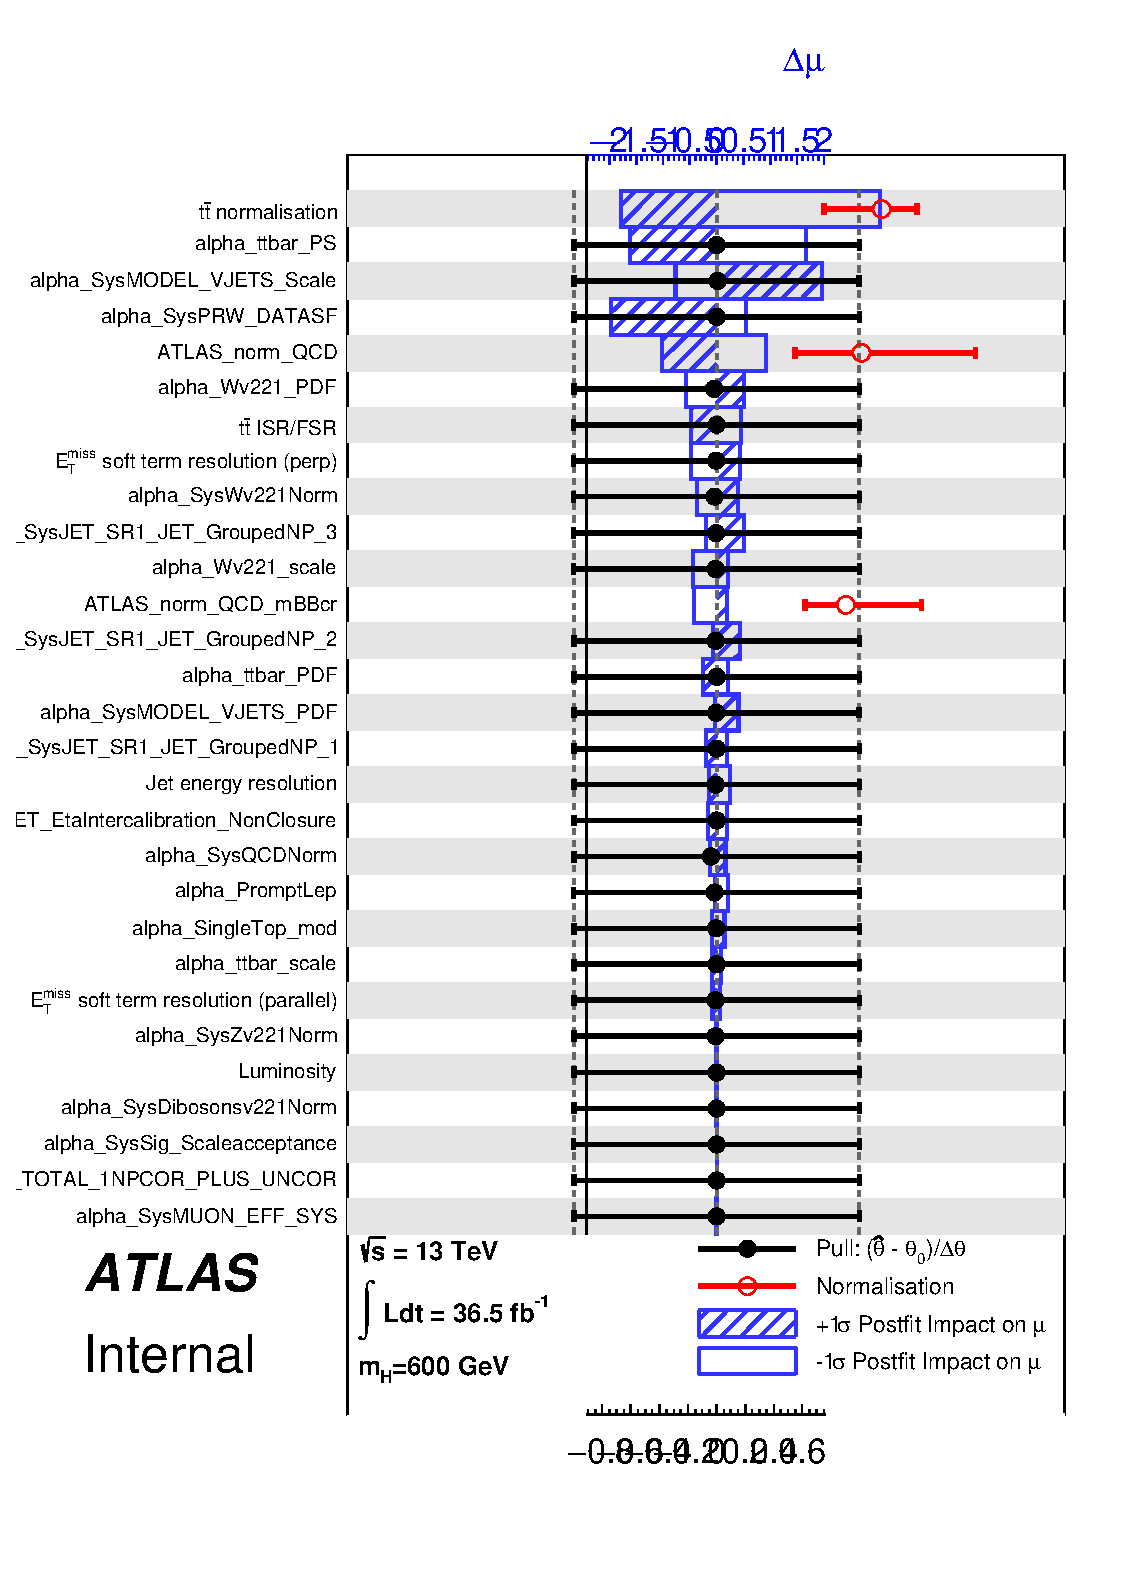
\includegraphics[height=60mm]{figures/statFit_appendix/pullPlot_X600_mu0_unconditional.eps} 
  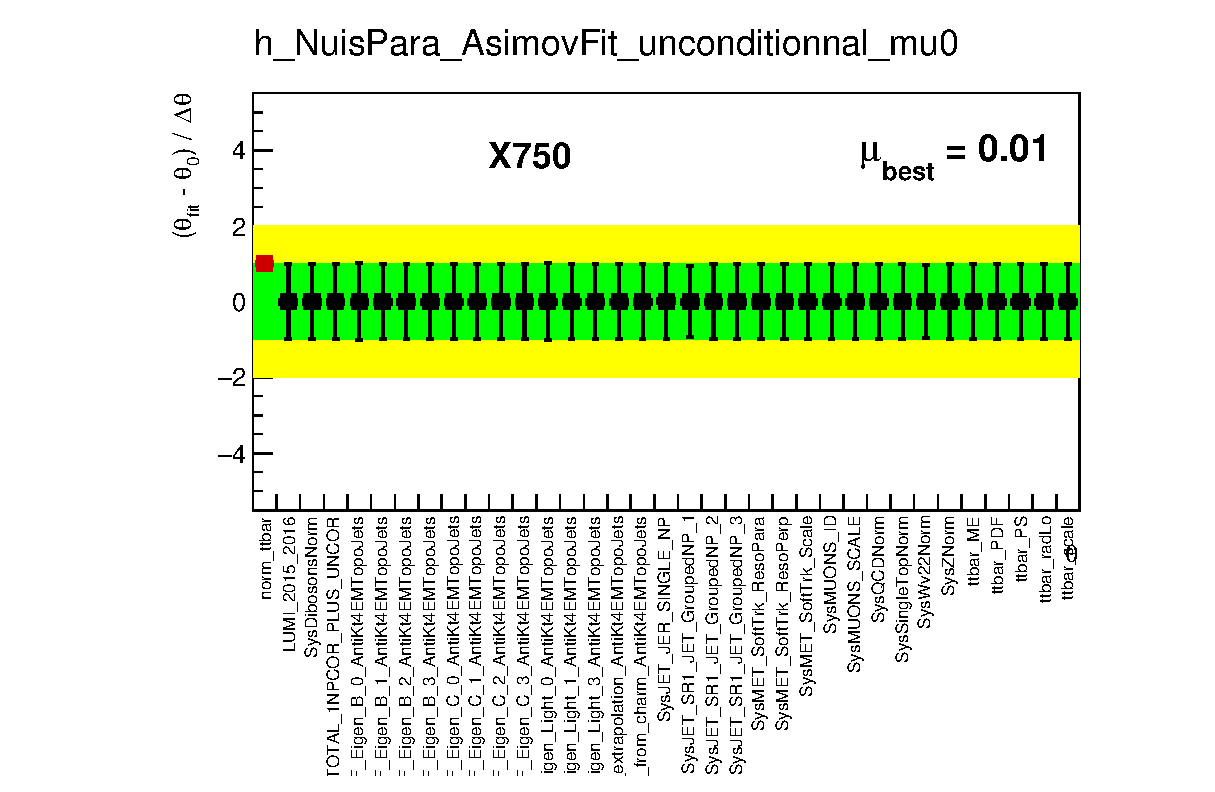
\includegraphics[height=60mm]{figures/statFit_appendix/pullPlot_X750_mu0_unconditional.eps}
  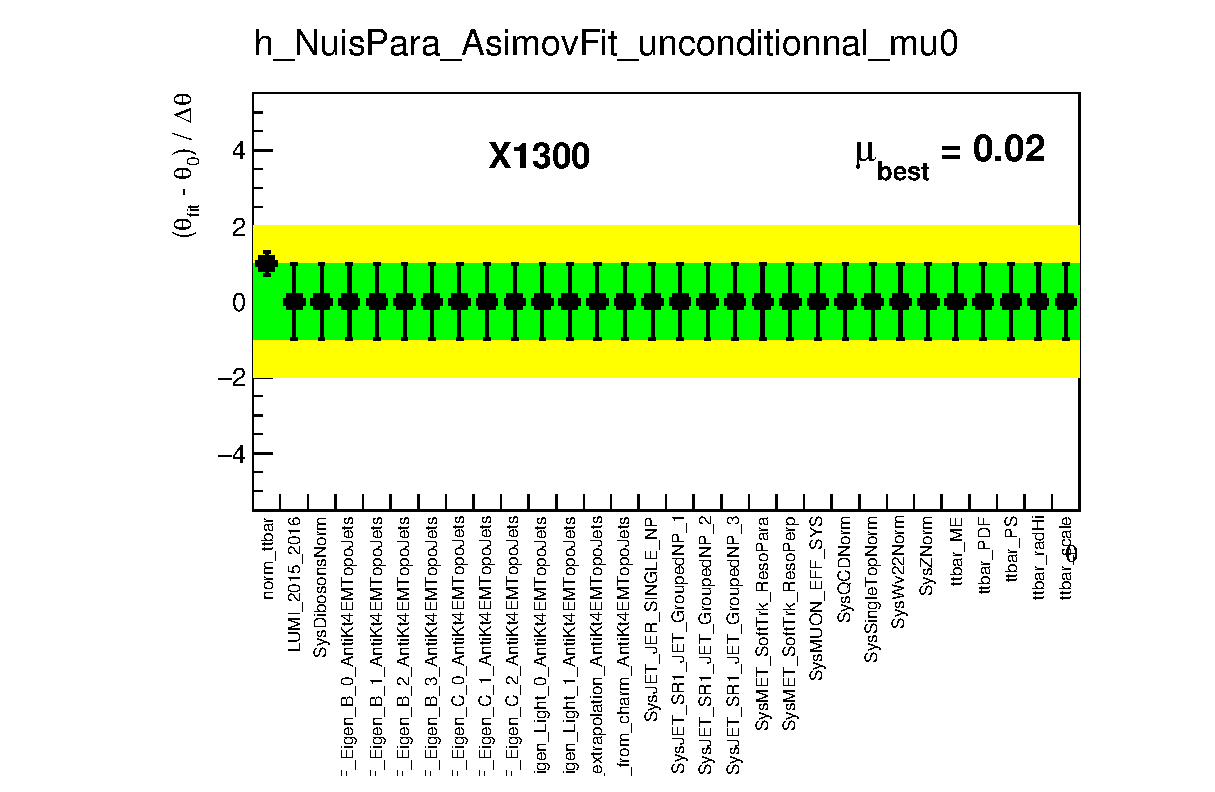
\includegraphics[height=60mm]{figures/statFit_appendix/pullPlot_X1300_mu0_unconditional.eps}
  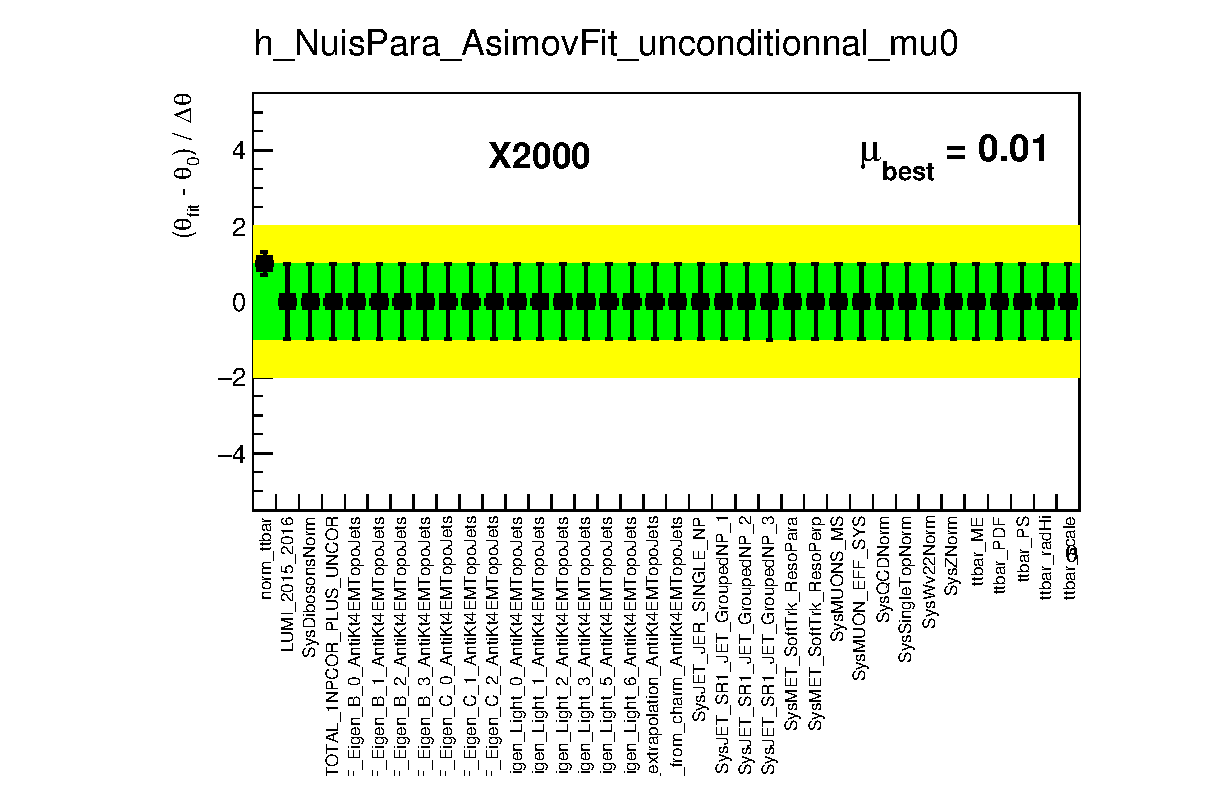
\includegraphics[height=60mm]{figures/statFit_appendix/pullPlot_X2000_mu0_unconditional.eps}
  \caption{Pull plots produced when fitting to an Asimov dataset created and profiled at $\mu=0$ for m$_X$ = 600, 750, 1300, and 2000 GeV. In the fit, $\mu$ is allowed to float as a free parameter.}
  \label{fig:pullPlots_mu_uncond}
\end{center}    
\end{figure}
%%%%%%%%%%%%%%

\begin{figure}[hb]
\begin{center}
  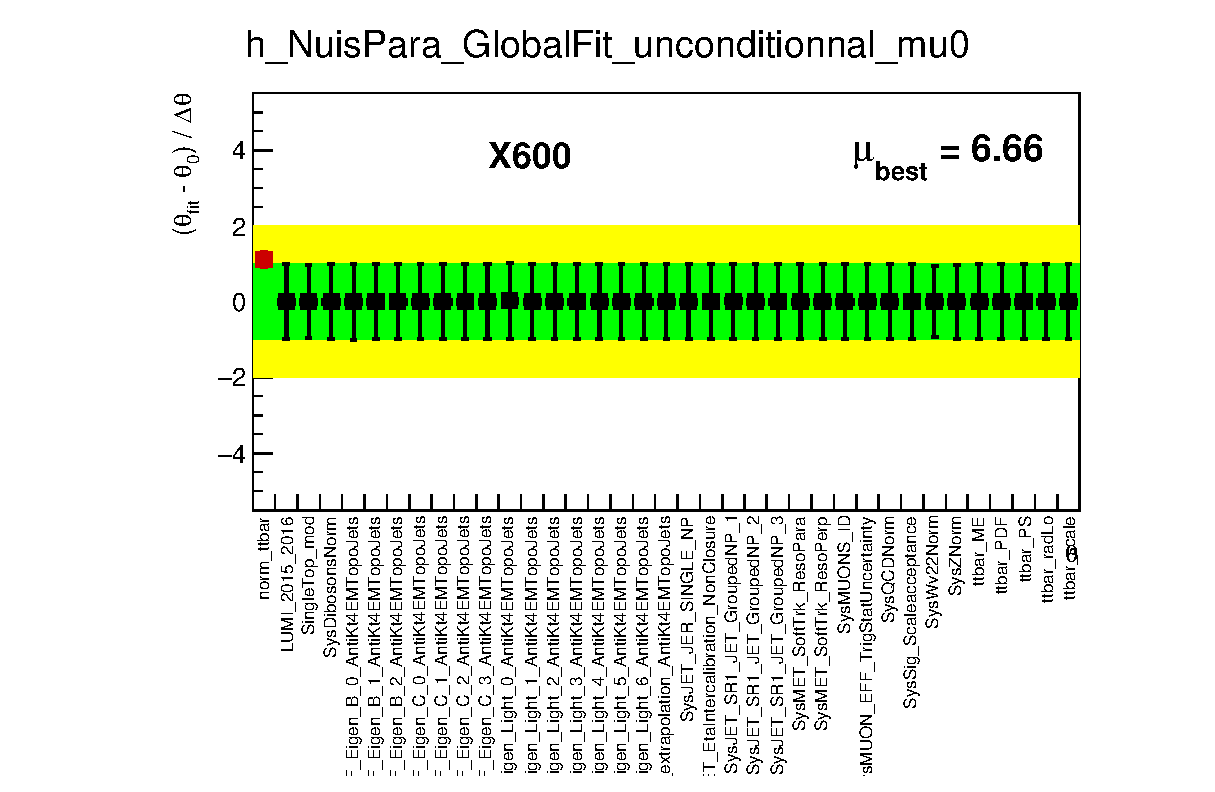
\includegraphics[height=60mm]{figures/statFit_appendix/pullPlot_X600_globalFit_mu0_unconditional.eps} 
  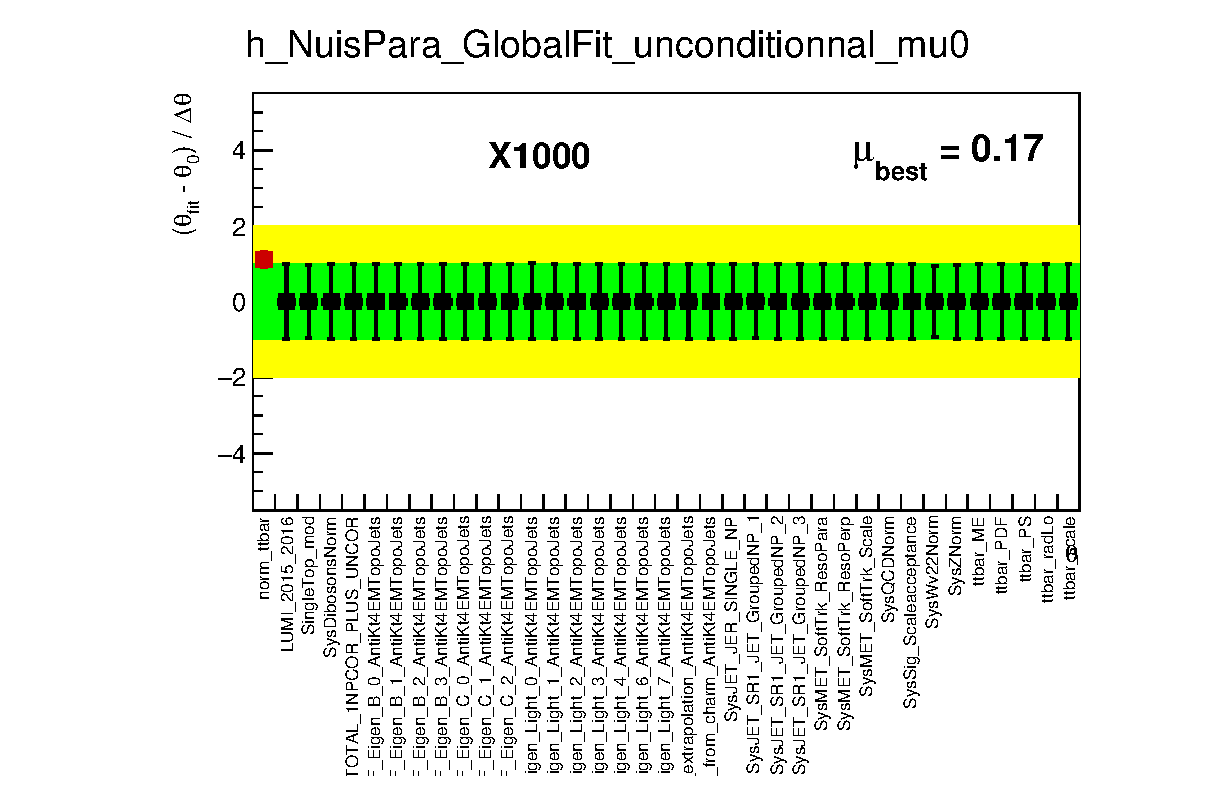
\includegraphics[height=60mm]{figures/statFit_appendix/pullPlot_X1000_globalFit_mu0_unconditional.eps}
  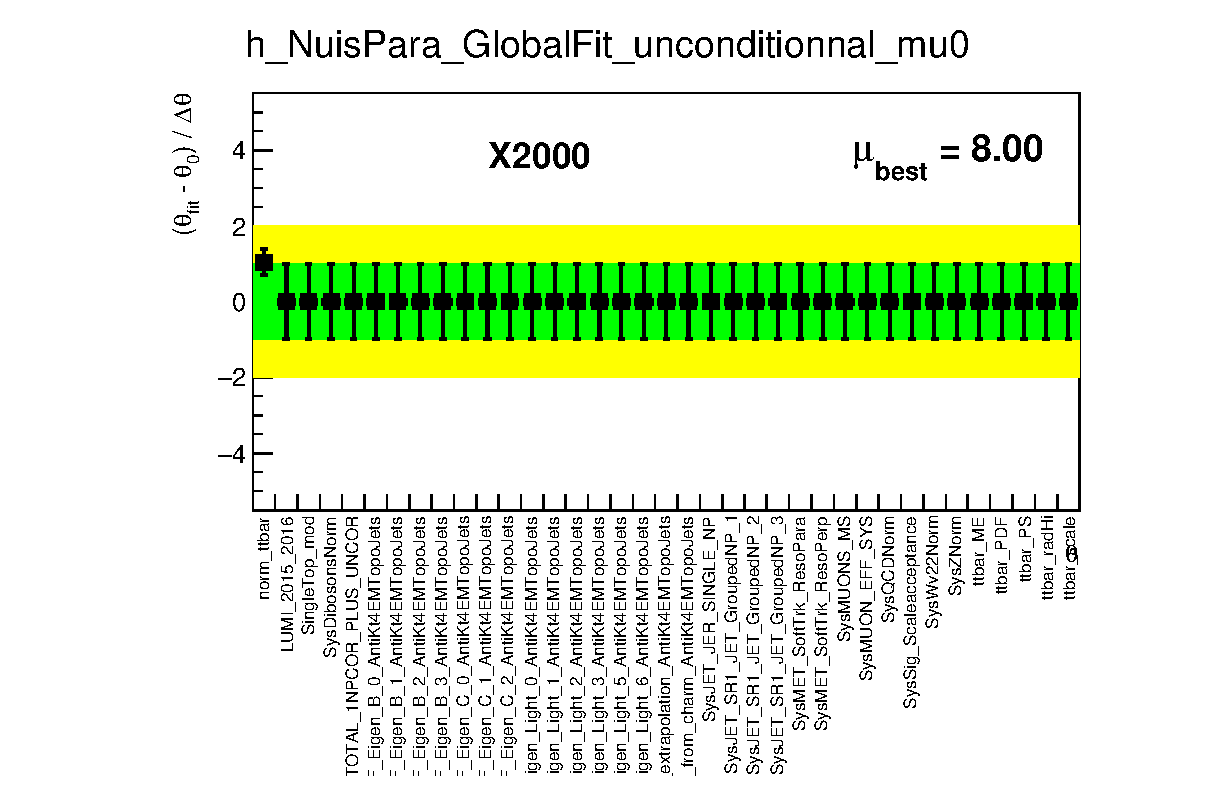
\includegraphics[height=60mm]{figures/statFit_appendix/pullPlot_X2000_globalFit_mu0_unconditional.eps}
  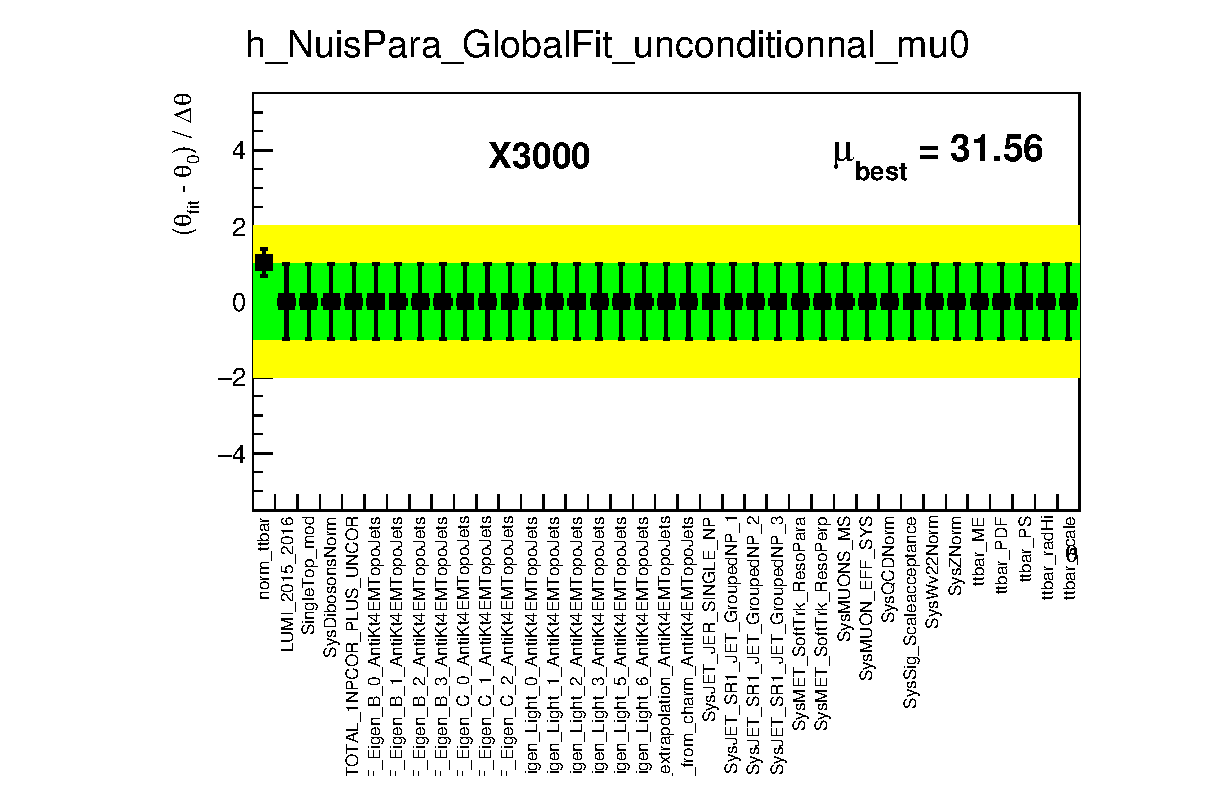
\includegraphics[height=60mm]{figures/statFit_appendix/pullPlot_X3000_globalFit_mu0_unconditional.eps}
  \caption{Pull plots produced with observed dataset  for m$_X$ = 600, 1000, 2000, and 3000 GeV. In the fit, $\mu$ is allowed to float as a free parameter.}
  \label{fig:pullPlots_mu_uncond_obs}
\end{center}    
\end{figure}
%%%%%%%%%%%%%%

%\begin{figure}[hb]
%\begin{center}
%  \includegraphics[width=.75\textwidth]{figures/statFit_appendix/90011_140916-v0-hiMassRankingAndPulls-x1300_HH_13TeV_140916-v0-hiMassRankingAndPulls-x1300_Systs_1300_pulls_1300}
%  \caption{NP ranking plot for m$_X = 1300$ GeV produced when fitting to data in the control region and psuedodata built from Monte Carlo in the signal region.}
%  \label{fig:npRanking_1300}
%\end{center}    
%\end{figure}

%\begin{figure}[hb]
%\begin{center}
%  \includegraphics[width=.75\textwidth]{figures/statFit_appendix/90014_140916-v0-hiMassRankingAndPulls-x2000_HH_13TeV_140916-v0-hiMassRankingAndPulls-x2000_Systs_2000_pulls_2000}
%  \caption{NP ranking plot for m$_X = 2000$ GeV produced when fitting to data in the control region and psuedodata built from Monte Carlo in the signal region.}
%  \label{fig:npRanking_2000}
%\end{center}    
%\end{figure}
